Wykorzystywane w optyce materiały charakteryzują się niską podatnością magnetyczną w rozważanej części widma, w związku z czym przyjmuje się $\mu(\omega)=1$. Ze względu na właściwości elektryczne wykorzystywane materiały możemy  podzielić na dielektryki~i przewodniki. Dielektrykami nazywamy materiały,~w których pod wpływem zewnętrznego pola elektrycznego powstają dipole elektryczne. Powodem powstawania dipoli może być przesunięcie ładunków dodatnich w stusunku do ujemnych lub powstanie spójnej orientacji przestrzennej dipoli elektrycznych tworzących dany ośrodek. W przeciwieństwie do dielektryków, ze względu na obecność swobocnych nośników ładunku elektrycznego przewodniki nie ulegają polaryzacji w zewnętrznym polu elektrycznym. W niniejszej pracy jako przewodniki rozważane są metaliczne pierwiastki chemiczne, dlatego terminy przewodnik i metal traktowane są zamiennie.

\begin{figure}[tb]
	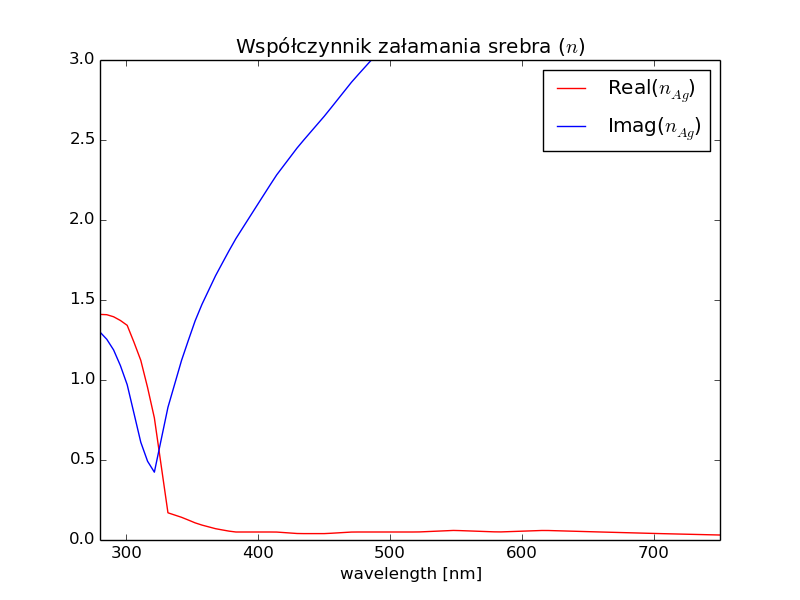
\includegraphics[width=\textwidth]{images/agn.png}
	\caption{Zależność współczynnika załamania od długości fali w zakresie optycznym, dla metalu - $Ag$ \cite{PhysRevB.6.4370}.  }
	\label{fig:agn}
\end{figure}
Zjawiska fizyczne omawiane w poniższym rozdziale bardzo silnie zależą od przenikalności elektrycznej wykorzystywanych materiałów. W szczególności wymagają wykorzystywania materiałów o ujemnej przenikalności elektrycznej. Takie własności przejawiają metale, których zastosowanie do nadrozdzielczego obrazowania przy pomocy cienkiej warstwy przewodnika zaproponował John Pendry. Wykorzystanie warstwy znacznie cieńszej od dłgości fali pozwala na rozsprzężenie pola elektrycznego i magnetycznego przez co możliwe jest nadrozdzielcze obrazowanie przy pomocy materiału z $\mu=1$. \cite{PhysRevLett.85.396}

\begin{figure}[tb]
	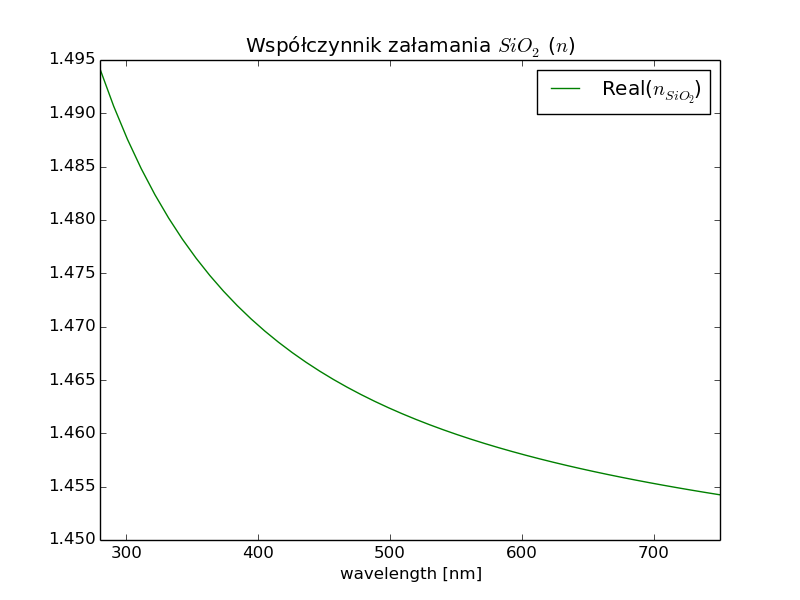
\includegraphics[width=\textwidth]{images/sio2n.png}
	\caption{Zależność współczynnika załamania od długości fali w zakresie optycznym, dla szkła kwarcowego -  $SiO_2$ \cite{MALITSON:65}   }
	\label{fig:sio2n}
\end{figure}
W zakresie optycznym znajdują się częstości rezonansowe atomów metali skutkujące silną dyspersją współczynnika załamania i wysoką absorpcją. Zależność rzeczywistej i urojonej części współczynnika załamania  dla srebra prezentuje wykres \ref{fig:agn}. Na wykresie widać charakterystyczny obszar w zakresie ok. 310-350 nm w którym obserwujemy znaczny spadek części rzeczywistej współczynnika załamania i minimum zdolności absorbcyjnych. Wysoka wartość części urojonej współczynnika załamania wskazuje na silną absorbcję promieniowania dla długości fali powyżej 350nm.

Dla dielektryków współczynnik załamania zazwyczaj maleje wraz ze wzrostem długości fali. Zależnośc ta jest znacznie słabsza niż w przypadku metali. Jako przykład na wykresie \ref{fig:sio2n} przedstawiono współczynnik załamania $SiO_2$. Urojona część współczynnika załamania dla dielektryków jest mniejsza niż w przypadku metali. W~szczególnośc dla przedstawionego szkła kwarcowego w większości zastosowań jest zaniedbywana.

\begin{figure}[tb]
	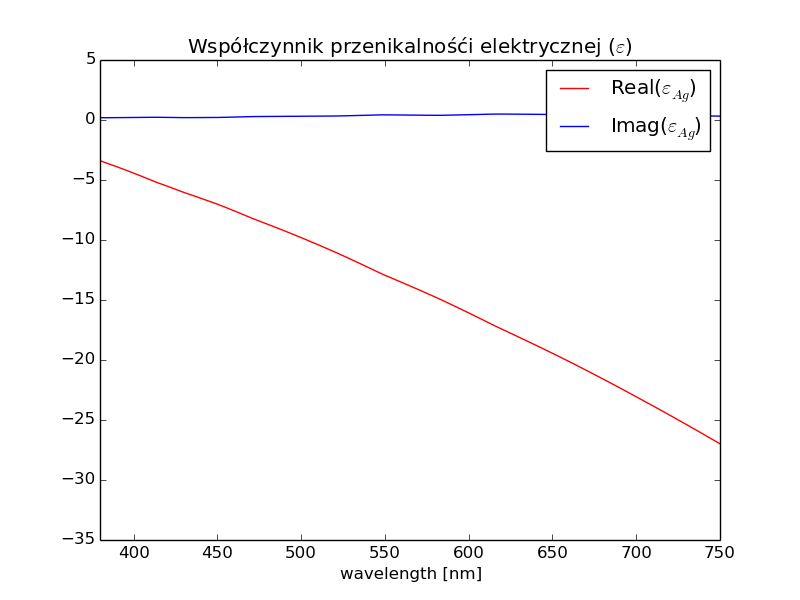
\includegraphics[width=\textwidth]{images/agtio2eps.png}
	\caption{Zależność przenikalności elektrycznej od długości fali w zakresi optycznym, dla metalu $Ag$ \cite{PhysRevB.6.4370} }.  
	\label{fig:agtio2eps}
\end{figure}
W celu opisu dyspersyjnych dielktryków z~powodzeniem stosuje się model Lorenza-Lorenza, a~wartość $\varepsilon$ często traktowana jest jako stała. W przypadku metali, ze względu na wspomniany charakter rezonansowy $\varepsilon(\omega)$  musi być opisywana przy użyciu modelu Lorenza-Drudego. Dokładniejsze omówienie tego modelu znajduje się w rozdziale \ref{subart:lorenz-drude}.

Należy zaznaczyć, że pominięty został wpływ wektora falowego na wartości $\varepsilon$ i $\mu$. W ogólności $\varepsilon(\omega,\vec{k})$ jest funkcją zarówno częstotliwości jak i wektora falowego, co należy rozumieć jako zależność indukcji elektrycznej $\vec{D}(t,\vec{r})$ nie tylko od wzbudzenia w poprzedzającej chwili czasu $t'$, ale również od wzbudzenia fali elektromagnetycznej w otoczeniu $\vec{r'}$. Ze względu na zależność od otoczenia ta klasa zjawisk nazywana jest nielokalnymi. Wpływu otoczenia na stan polaryzacji $\vec{P}$ nie można pomijać gdy zmienność pola elektromagnetycznego jest znacząca w porównaniu z drogą swobodną elektronów w ośrodku.



